%******************************************************************************************************
\chapter[Introduction]{Quantifying Uncertainty of Computer Model: Forward and Backward}\label{ch:intro}
%******************************************************************************************************

% Introductory Paragraphs
In this opening chapter, some his chapter describes an approach to construct a fast surrogate model (metamodel) that approximates (or emulate) the input/output relationship of an expensive code for faster evaluation at any given input parameters values located in the specified domain.
As argued in Section~\ref{sub:intro_statistical_metamodeling} this thesis used the one based on Gaussian stochastic process which results in a statistical metamodel. 

% Overview of the chapter
This opening chapter intends to introduce briefly the importance, the use and the challenges of using system code in simulating thermal-hydraulics behavior of \gls[hyper=false]{npp} in the context of its safety analysis.
Section~\ref{sec:intro_computer_simulation} 
It also defines the relevant terms used throughout the thesis.
The uncertainty analysis is first introduced in Section~\ref{sec:intro_uncertainty_quantification}.
The section also provides the context of the present doctoral research.

% Objectives, Scope, and Statistical Framework
Section~\ref{sec:intro_objectives_and_scope} then describes the statement of the problem followed by objectives and scope of the research.
This thesis proposed a methodology comprises of three sequential steps to analyze a computer model with the overall goal to quantify the uncertainty.
It consolidates and adapts recent developments of in the applied statistics literature.
In relation to that, Section~\ref{sec:intro_statistical_framework} provides a broad overview of the research landscape on each of the proposed steps.
Finally, Section~\ref{sec:intro_thesis_structure} briefly outlines the structure of the thesis.

%************************************************************************************************************
\section{Computer Simulation and Safety Analysis of Nuclear Power Plant}\label{sec:intro_computer_simulation}
%************************************************************************************************************

The ubiquity of computer simulation applications in many fields of science and engineering results in an even more pervasive definitions of the term \textit{scientific computer simulation} itself 
and other associated terms such as \textit{model} and \textit{simulation}.
\marginpar{scientific computer simulation}
Though most of the definitions in the literature are not necessarily in contradiction to each other, 
to avoid confusion, this thesis adopts a recent definition proposed by Kaizer et al.\cite{Kaizer2015} quoted below,

\begin{quote}
	Scientific Computer Simulation is the imitation of a behavior of a system, entity, phenomenon, or process in the physical universe 
	using limited mathematical concepts, symbols, and relations through the exercise or use of scientific computer model.
\end{quote}

There are three main points highlighted in this definition.
\marginpar{model, simulation, and computer simulation}
First, this definition accentuates the difference between a \emph{model} and its \emph{simulation}.
Specifically, the former deals with the notion of representation, while the latter deals with the notion of imitation of a behavior.
Secondly, what makes a model scientific is that it treats physical phenomena or the behavior of a real world system as its subject.
Thirdly and finally, the modifier \emph{computer} in the definition makes it explicit that digital computer is used to solve whatever mathematical models serve as the representation.
This is usually the case for mathematical models that cannot be solved analytically.
Though this limitation what makes a solution of the model possible in the first place, 
it also affects the solution and its possible interpretation and thus many computational-related aspects also need to be comprehensively considered.
\footnote{Beven \cite{Beven2009} articulates this distinction into three levels of model: perceptual model (i.e., theoretical description of some physical phenomena), formal model (i.e., the mathematical description of it), and procedural model  (i.e., computer implementation of the formal model). For many physical system modeling applications, only the procedural model is able to make a quantitative prediction of the system. These distinctions are useful in acknowledging the level of approximation involved in moving from perceptual to procedural model.}
%*************************************************************************************************************************
\section{Uncertainty Quantification in Nuclear Engineering Thermal-Hydraulics}\label{sec:intro_uncertainty_quantification}
%*************************************************************************************************************************

% Introductory Paragraph
Before continuing the discussion of uncertainty analysis of code predictions, it will be worthwhile to define some additional terminologies to avoid later confusion.

In making a connection with the notion of \emph{simulator} introduced in Section~\ref{sec:intro_computer_simulation}, 
recall that from Fig.~\ref{fig:ch1_th_system_code} an \emph{input deck} is distinct from the code itself.
Fig.~\ref{fig:ch1_simulator_io} depicts the notion of simulator of a thermal-hydraulics system in a more generic way, as an input/output model.
\begin{figure}[bth]	
	\centering
	\includegraphics[width=\textwidth]{../figures/chapter1/figures/simulator_io}
	\caption[Simplified illustration of a simulator as an input/output model.]{Simplified illustration of a simulator as an input/output model.}
	\label{fig:ch1_simulator_io}
\end{figure}

Indeed input deck defines specific problem (i.e., system) of interest.
It includes the specifications for geometrical configuration (i.e., the nodalization), choice of material and fluid involves, as well as initial and boundary conditions.
It may also include the setting for the numerical solver.
Some of those specifications (such as the boundary conditions, etc.) are parametrized and constitutes \emph{controllable inputs} denoted by $\bm{x}_c$\footnote{later on, \emph{controllable} inputs corresponds to the equivalent parameters in a physical experiment which can be controlled by the experimentalist.}.
The conservation equations of the code are closed with additional set of closure laws (and other sub-models) $\mathcal{M}_i(\bm{x}_c, \bm{x}_m, \bm{u})$.
These closure laws are, in turn, parametrized with a set of model specific parameters denoted by $\bm{x}_m$ which is referred to as the \emph{physical model parameters}.
 
Specifying the input deck, as far as user is concerned, completely defines the problem and the code will solve the conservation equations which output the dynamic state of relevant physical variables $\mathbf{u}(\bm{r}, t)$ (e.g., fluid pressure, temperature, wall temperature, etc.).
In practice, these raw simulation outputs are further post-processed to obtain the so-called \glspl[hyper=false]{qoi} the are relevant to the problem at hand.

%--------------------------------------------------------------------------
\subsection{Forward Uncertainty Quantification}\label{sub:intro_uq_forward}
%--------------------------------------------------------------------------

% Best-estimate, limitation
As explained, best-estimate analysis uses more realistic modeling assumptions for analyzing transient behavior of \gls[hyper=false]{npp}.
It attempts as realistically as possible to describe the behavior of the relevant physical processes occur during the plant transient.
And yet, even the best available understanding of the physical process is still limited.
Understanding of complex phenomena might not yet adequate and data support for some processes can be very limited.s
Simplifying assumptions, approximations, and expert judgments to some degree are unavoidable and still required to have a complete analysis.

% Best-estimate, plus uncertainty
Hence, best-estimate analysis has to be complemented with uncertainty analysis.
\marginpar{Best-estimate plus uncertainty}
The ultimate goal of uncertainty analysis is to associate code prediction with its uncertainty.
These combined quantities are then compared with certain regulator safety limits (e.g., \gls[hyper=false]{pct}) to check whether the limits still fall outside the uncertainty band of the code prediction.

% Source of possible uncertainties
There are several known sources of uncertainty that render the prediction on $\bm{u}(\mathbf{r},t)$ and its derived quantities uncertain.
The following are the sources of primary interest in the present research:
\begin{enumerate}
	\item 1 
  \item 2
  \item 3
\end{enumerate}

% Forward uncertainty quantification, Inputs as random variables
In statistical uncertainty analysis, the controllable inputs and physical model parameters are modeled as random variables ($\bm{\mathcal{X}}_c$ and $\bm{\mathcal{X}}_m$, respectively) equipped with probability distributions.
\marginpar{Forward uncertainty quantification}
Then using \gls[hyper=false]{mc} technique, samples are generated from their respective distributions and they are used to run the code multiple times.
Finally, statistics of code outputs (raw or post-processed), are summarized to obtain the uncertainty measure of the prediction.
In other words, the uncertainties in the controllable inputs and physical model parameters are \emph{propagated forward} through the code to quantify the uncertainty of the predictions as shown in Fig.~\ref{fig:ch1_simulator_uq_forward}.
The practice of propagating uncertainty by \gls[hyper=false]{mc} is widely accepted in the nuclear engineering thermal-hydraulics community \cite{Lellouche1990,Glaeser1994,Glaeser2008}.
\begin{figure}[!bth]	
	\centering
	\includegraphics[width=\textwidth]{../figures/chapter1/figures/simulator_uq_forward}
	\caption[Simplified flowchart of forward uncertainty quantification of a simulator prediction.]{Simplified flowchart of forward uncertainty quantification of a simulator prediction. Notice that the simulator has been parametrized by the controllable inputs and physical model parameters, each of which are represented as random variable.}
	\label{fig:ch1_simulator_uq_forward}
\end{figure}

% Source of uncertainty, initial and boundary condition

% Source of uncertainty, physical model parameters

% Model parameters
The physical model parameters, however, are conceptually different.
\marginpar{Model parameters}
The physical models referred to in this thesis are usually represented either in the form of correlation or phenomenological (mechanistic) model.
The parameters associated with these models are derived from experimental data.
They can either represent physically meaningful quantities (e.g., reaction rate coefficient) or not (i.e., a tuning parameter).
In either way, there are uncertainties associated with these parameters especially as the conditions of their intended use is making prediction can be (at times, very) different than the conditions of their derivation.
The conceptual distinction related to model parameters will be revisited in Chapter~\ref{ch:bayesian_calibration}.

%--------------------------------------------------------------------------
\subsection{Inverse Uncertainty Quantification}\label{sub:intro_uq_inverse}
%--------------------------------------------------------------------------

% Introductory paragraph, motivation
The physical model parameters often cannot be measured directly.
In this situation, in order to estimate their values,
experiments with well-specified conditions are carried out and correlations (models) are fitted based on the experimental data. 
Recall that from the discussion of closure laws origin in Section~\ref{sub:intro_th_system_code},
this can also apply to phenomenological models where free parameters are allowed to be tuned according to match the experimental data.
Ultimately, the optimal value of the estimated parameter is implemented in the code.
As the code is used to simulate multiple phenomena during a transient, additional experiments are carried out in larger, more complex test facilities.
Finally, based on the data obtained, the models can be validated.

% Inverse uncertainty
To obtain the uncertainty associated with the model parameters obtained in the manner above, the problem can be posed as an inverse problem.
In this setting, given a set of experimental data $\{\mathbf{D}\}$ with a known controllable inputs $\mathbf{x}_c$, the task is then to infer the value of the physical model parameters.
It is important to acknowledge various sources of uncertainty previously mentioned:
experimental data and controllable inputs are observed but perhaps there remains residual uncertainty and observation error associated with them;
and the associated models are also only an approximation of the real physical processes with a possible, but unknown, systematic bias.
\bigfigure[pos=tbhp,
           opt={width=1.0\textwidth},
           label={fig:ch1_simulator_uq_inverse},
           shortcaption={Simplified flowchart of inverse uncertainty quantification of model parameters.}]
{../figures/chapter1/figures/simulator_uq_inverse}
{Simplified flowchart of inverse quantification for model parameters of a simulator.}

% Connection to PREMIUM Benchmark
The importance of characterizing the uncertainty in the physical models parameters was acknowledged by the \gls[hyper=false]{wgama} of the \gls[hyper=false]{oecd}/\gls[hyper=false]{nea}.
This led to the \gls[hyper=false]{premium} project.
Its main goal is to report the state-of-the-art of the available methodologies to quantify the uncertainty in the physical models parameters.
The following will briefly describe the project and highlight its main findings.

%-------------------------------------------------------------
\subsection{OECD/NEA PREMIUM project}\label{sub:intro_premium}
%-------------------------------------------------------------

% Introductory paragraph
The \gls[hyper=false]{premium} project was an activity launched by the \gls[hyper=false]{oecd}/\gls[hyper=false]{nea} in $2012$ and concluded in $2016$ with the aim to advance the methods for quantifying the uncertainties associated with the physical model parameters in \gls[hyper=false]{th} system codes.
It was the continuation of the previous project \gls[hyper=false]{bemuse}, which concetrated on the propagation and sensitivity analysis of the input uncertainties in large scale simulation (large break \gls[hyper=false]{loca}).
The main finding of \gls[hyper=false]{bemuse} can be found in \cite{Perez2011}.
The emphasis of the \gls[hyper=false]{premium} benchmark was placed on the derivation of the model parameters uncertainty and their validation.

% Scope of the Project

% Main Findings

%*********************************************************************************
\section{Objectives and Scope of the Thesis}\label{sec:intro_objectives_and_scope}
%********************************************************************************* 

With a larger context provided above,
this section presents briefly and specifically the statement of the problem,
followed by the objectives as well as the scope of the present doctoral research.

%--------------------------------------------------------------------------
\subsection{Statement of the Problem}\label{sub:intro_statement_of_problem}
%--------------------------------------------------------------------------

% Introductory Paragraph
The development of closure laws for reflooding described in \cite{Nelson1992,USNRC2012} showed the difficulties and the amount of assumptions used.
In a nutshell, system code development is an effort to consolidate correlations and mechanistic models, to create a phenomenological-based simulation code that can provide best-estimate results.
This consolidated effort results in a code that can simulate wide range of transients foreseen in nuclear power plant operation in a best-estimate manner.
Alas, to come up with a consistent set of closure laws is a great challenge for code developers.

% Closure Laws Difficulty, Conceptual
The closure laws required to close the two-fluid model pose particularly difficult challenges \cite{Wulff2007}.
For instance, to have a correlation of heat transfer between the wall and the fluid, temperature data from each of the constituents are needed (i.e., the wall, the liquid phase, and the gas phase).
But measuring temperature of the individual phases in an arbitrary interfacial topology has its own technical difficulties to the extend that no such data exists or available to be implemented in the closure laws.
Additionally, the experiments to obtain hydrodynamic closure laws (e.g., interfacial friction factor, wall friction factor, etc.) were generally carried out in adiabatic conditions.
As a result, this excludes the coupling of any heat transfer phenomena between the phases and the wall in such correlation.

% Closure Laws Difficult, Practical
Furthermore, during the development of a simulation code, programming considerations also came into the picture.
For robustness, simplification is often required and continuity is enforced.
Transitionary flow regime between two known (observed) flow regimes for which experimental data is not available is modeled to be the average of the two bounding regimes.
Different code development, which used different assumptions and experimental database, comes up with different set of closure laws with their own parametrization (see for instance \cite{Nelson1992} for TRAC code and \cite{Bestion1990} for CATHARE code).
Several authors have expressed their concerns about the uncertainty stemming from the closure laws \cite{Wulff2007,Petruzzi2008a,DAuria2012}.

% an Illustration
As an example of the point given above, consider that in the \gls[hyper=false]{trace} code, after some derivations the interfacial drag coefficient closure law in the inverted slug flow regime $C_{i,\text{IS}}$ is given by,
\begin{equation*}
	C_{i,\text{IS}} = \hat{x}_{m,\text{SET}} \times \frac{1}{24} \frac{\rho_g}{\text{La}} \frac{(1-\alpha)}{\alpha^{1.8}} \,\,\,;\,\,\, \hat{x}_{m,\text{SET}} = 0.75 
\label{eq:intf_drag_isf}
\end{equation*}
where $\rho_g$ is the density of the gas phase;
$\text{La}$ is the Laplace number;
$\alpha$ is the void fraction;
and $\hat{x}_{m,\text{SET}}$ is a fitting parameter.

There are several remarks about the closure law given above.
First, the second term in the right-hand side was derived from experimental data but not directly.
In the inverted slug regime, saturated liquid core breaks up into ligaments.
These ligaments are \emph{assumed} to take form as prolate ellipsoid.
The drag coefficient of distorted droplet experimental database is then \emph{assumed}.
Then to take into account the multi-particle effect, the coefficient is divided by the void fraction $\alpha$ raised to the power of $1.8$ (this, in turn, was taken from experimental data of inertial regime).
Lastly, the first term of the equation, $\hat{x}_{m,\text{SET}} = 0.75$ was put \emph{to match}, \emph{to calibrate against} the experimental data from the FLECHT-SEASET reflood facility.
This first term, although clearly \emph{non-physical}, is an important tuning parameter of the model nevertheless.
Its uncertainty should be considered in uncertainty analysis, especially when reflood is expected to occur.
Yet, no statement regarding the associated uncertainty is given.
Several other such terms exist \cite{USNRC2012}. 

% Statement of Problem
As illustrated above, it is clear that models in thermal-hydraulics system code, to a certain extent, flawed.
Various experimental programs were carried out to gain better understanding of important phenomena,
and to validate (and, as noted above, to calibrate) the models.
Series of the experiments, carried out in \glspl[hyper=false]{setf} were aimed to reproduce limited part of the transient in a selected component following a postulated scenario.
For example, in the case of reflooding, several facilities existed and data were available (FEBA, PERICLES, etc.).
But, there has not been an orchestrated effort to incorporate the accumulated data into the calibration process of the physical models, in a systematic way, while acknowledging multiple sources of the uncertainty in the process.

%--------------------------------------------------
\subsection{Objectives}\label{sub:intro_objectives}
%--------------------------------------------------

% Introductory (Overall Objective)
The purpose of the doctoral research is to quantify the uncertainty of physical model parameters
implemented in a thermal-hydraulics system code.
The physical models of interest describe the phasic interactions in a complex multiphase flow during a reactor transient, namely heat, mass, and momentum exchanges between vapor, water and structures.
These models are parametrized by physical or empirical tuning parameters, the values of which are uncertain.
This results in uncertain code prediction of important safety quantities, such as the evolution of the fuel cladding temperature during a postulated reactor transient.

Adopting probabilistic framework to conform to the statistical uncertainty propagation widely
adopted in the field of nuclear engineering, the uncertainties in the parameters are represented in
form of probabilistic density functions or their approximation.
The derivation of these functions is posed as an inverse statistical problem following Bayesian framework as the parameters themselves are not directly observable.
The doctoral research thus aims to present a consistent set of strategies in deriving the uncertainty of such model parameters based on experimental data.
This is done by consolidating and adapting recent developments in the applied statistics literature:

% Aim 1 (Global sensitivity analysis)
\begin{enumerate}
	\item \emph{to analyze and to better understand} the inputs/outputs relationship in a computer simulation with uncertain inputs.
	This is aimed at answering the question whether the current physical model in thermal-hydraulics system code \gls[hyper=false]{trace} can be identified with the available experimental data from test facilities.
	In other words, how to select important parameters to be inferred.
	\Glsfirst[hyper=false]{gsa} methodologies can be used to assist in identifying which parameters can be calibrated using the available data.
	A test facility might have multiple types of data and although the information content might not be the same for the different types, it might be worthwhile to consider each one of them.
	Finally, for each of the different types,
	the analysis is also conducted on various derived \glspl[hyper=false]{qoi}, some of which explicitly consider the output as function.
	By doing so, it is hope that interesting model behavior with respect to its parameters perturbation can be revealed.

% Aim 2 (Statistical Metamodeling)
	\item \emph{to approximate} the inputs/outputs relationship in a complex computer simulation for a faster evaluation.
	The step is required as the statistical calibration method adopted in thesis is computationally expensive, requiring numerous code runs in the order of hundreds of thousands and beyond.
	This approximation is done through a \glsfirst[hyper=false]{gp} metamodel resulting in a statistical metamodel.
	The highly multivariate nature of the outputs (time- and space-dependent) is dealt by a dimension reduction technique.
	Build upon the results of previous step, only parameters that are identified to be influential are included in the construction of the metamodel.

% Aim 3 (Bayesian Calibration)
	\item \emph{to statistically calibrate} the physical model parameters against various relevant experimental data.
	The word \emph{to calibrate} carries a disparaging interpretation related to \emph{to tweak}.
	However, using a Bayesian statistical framework, the aim of calibration is extended to simultaneously quantify the uncertainty of the parameter estimation.
	The framework includes various sources of uncertainty which can be modeled using probabilistically, including the model bias term.
	At the end, the parameters of interest will be either in the form of distributions conditioned on the data or samples generated from such distributions which are useful in the uncertainty analysis of code prediction.

% Aim 4 (Extrapolation)
	\item \emph{to validate} the statistical calibration results against experimental data set not used in the calibration step.
	As calibration only conducted using experimental data of limited experimental conditions, it is important, at the minimum, to validate the proposed methods by demonstrating the applicability of the results to the simulation of the phenomena of the same facility in different experimental conditions. 

\end{enumerate}

%----------------------------------------
\subsection{Scope}\label{sub:intro_scope}
%----------------------------------------

% Introductory paragraph
Although the proposed set of strategies in this research can be applicable to the analysis and calibration of any system code physical model,
it is illustrated by its application on the models of particular importance during simulation of reflooding,
i.e., the so-called \gls[hyper=false]{postchf} flow regimes.
There are several reasons for this emphasis:
\begin{itemize}

	% Reason 1
	\item Reflooding is an important part in the simulation of \glspl[hyper=false]{npp} transient during \gls[hyper=false]{loca}.
	Modeling reflooding determines the appropriate representation of the dynamics of heat transfer phenomena during the effort to rewet an uncovered core.
	Of paramount interest is to estimate the time the rod can be expected to be rewet as well as the maximum temperature reached prior to rewet.
	Reflood is a transient with highly coupled hydrodynamic-heat-transfer effects and it challenges the assumption made on the implemented closure laws.
	Indeed several reflood experimental programs conducted in \glspl[hyper=false]{setf} existed and were designed to validate reflood models in system code.
	Unfortunately, no orchestrated effort was done so far to consolidate the generated data in general and into \gls[hyper=false]{trace} code in particular.

% Reason 2
	\item The models are adequately complex. It is complex that $5$ flow regimes are involved in a single phenomena: multiple sub-models, parametrized with numerous inputs, with multivariate outputs (both time- and space-dependent).
	But as the source of data is from reflooding \glspl[hyper=false]{setf}, real plant system (and full scale) effects can be excluded and the ensuing analysis can be concentrated on limited set of models.
	In fact, as already pointed out, reflooding \glspl[hyper=false]{setf} were designed to validate and (to calibrate) reflood models in system codes.

% Reason 3
	\item Multiple data of various types (taken with different experimental conditions) are typically available from experiment within the same facility.
	As calibration in the present research is conducted using one experimental condition, it is important to validate the resulting calibration result against the data with different experimental condition albeit from the same experimental facility. 
	Moreover, additional data from another reflooding \glspl[hyper=false]{setf} are also available.
	This is important for future study of validating the proposed method further and of expanding it to calibration against data from multiple facilities. 

% Reason 4
	\item It is the model considered in the \gls[hyper=false]{premium} benchmark, thus there is possibility to compare the results of this research with the results of other participants of the benchmark\footnote{at least qualitatively due to different codes employed by different participants}.
	
\end{itemize}

As such, while it is important to acknowledge that reflood simulation and the associated relevant model (or models) are only parts of a large and complex thermal-hydraulics systems code,
they can provide a representative and relevant illustration on the particulars of analyzing and calibrating a thermal-hydraulics system code using experimental data from \gls[hyper=false]{setf} in general; providing a suitable testing ground for the proposed methods.

% Closing
As a final note, the thermal-hydraulics system code considered in this thesis is the \glsfirst[hyper=false]{trace} code developed by the \glsfirst[hyper=false]{usnrc}.
The main reason to consider solely this particular code in the present thesis is the fact that \gls[hyper=false]{trace} is the thermal-hydraulics system code used for the purpose of Swiss nuclear power plant safety analysis conducted withing the \glsfirst[hyper=false]{stars} program \cite{PSI2017} at the \glsfirst[hyper=false]{psi}.
\section{Statistical Framework}\label{sec:gp_statistical_framework}
\newpage
%------------------------------------------------------------------
\section{Structure of the Thesis}\label{sec:intro_thesis_structure}
%------------------------------------------------------------------

This doctoral thesis is organized into six chapters.
The description and the application on a thermal-hydraulics simulation of the three statistical approaches introduced before,
preceded by a brief review on the \gls[hyper=false]{th} system code \gls[hyper=false]{trace} as well as the selected phenomenon of interest and the associated physical models,
constitute the main chapters of the present thesis (see Fig.~\ref{fig:ch1_methodological_roadmap}).
They are bookended by an introductory chapter (this chapter) and a concluding chapter.
\begin{figure}[bth]	
	\centering
	\includegraphics[width=\textwidth]{../figures/chapter1/figures/methodological_roadmap}
	\caption[The structure of thesis.]{The structure of the thesis, its main chapters.}
	\label{fig:ch1_methodological_roadmap}
\end{figure}

\textsc{Chapter~\ref{ch:trace_reflood}} gives an overview of the system thermal-hydraulics code \gls[hyper=false]{trace} with an emphasis on its reflood phenomena modeling and simulation.
The chapter also introduces the reflood experiment at the \gls[hyper=false]{feba} facility which serves as the experimental basis of this work followed by its modeling in \gls[hyper=false]{trace} code.
This model becomes the running case study in the three subsequent chapters to which the proposed methods are applied.
The chapter includes the selection of initial parameters relevant for reflood simulation and the propagation of their uncertainties on the code prediction.

\textsc{Chapter~\ref{ch:gsa}} introduces the \gls[hyper=false]{gsa} analysis methods adopted in this thesis with three key underlying ideas.
The first is to reduce the dimensionality of the code output space.
As the output of the simulation is time-dependent, dimension reduction is carried out while trying to preserve the interpretability of the results.
The second idea is to reduce the dimensionality of the input parameters space through parameter screening.
The third and final idea is to investigate, quantitatively, the effect of variation of parameters on the overall time-dependent output variation through variance decomposition.
The presented methods are then applied to the \gls[hyper=false]{trace} model of \gls[hyper=false]{feba} and the results are discussed. 

\textsc{Chapter~\ref{ch:gp_metamodel}} presents an approach to construct a fast surrogate model that approximates the inputs/outputs relationship of a computationally expensive simulator.
A minimum theoretical foundation of the method is first introduced, before moving on to describing an approach adapting the method for dealing with highly multivariate output via dimension reduction.
Afterward, the application of the method to the \gls[hyper=false]{trace} model of \gls[hyper=false]{feba} is presented and discussed.
In the end, a metamodel of the \gls[hyper=false]{trace} model is constructed and validated in anticipation of the high cost of the calibration approach presented in the following chapter.

\textsc{Chapter~\ref{ch:bayesian_calibration}} describes the Bayesian calibration, the last of the main chapters of the thesis.
The description of the methods are splitted into two parts, following the convention in the Bayesian data analysis, the formulation part and the computation part.
The formulation of the Bayesian statistical calibration problem (i.e., the posterior) as well as its simplification (the so-called \emph{modularization}) are first introduced.
The resulting posterior is potentially complex and high-dimensional \gls[hyper=false]{pdf}. 
Consequently, the computational part is focused on a simulation-based approach called \gls[hyper=false]{mcmc} to directly generate representative samples useful for downstream analysis (e.g., forward propagation).
After that, as the two previous chapters, the application of the method to the \gls[hyper=false]{trace} model of \gls[hyper=false]{feba} is presented and the results are discussed.
Included in the discussion is the validation of the method based on the additional experimental data of \gls[hyper=false]{feba} not used in the calibration.

\textsc{Chapter~\ref{ch:conclusions}}

%\begin{sidewaysfigure}
%	\centering
%	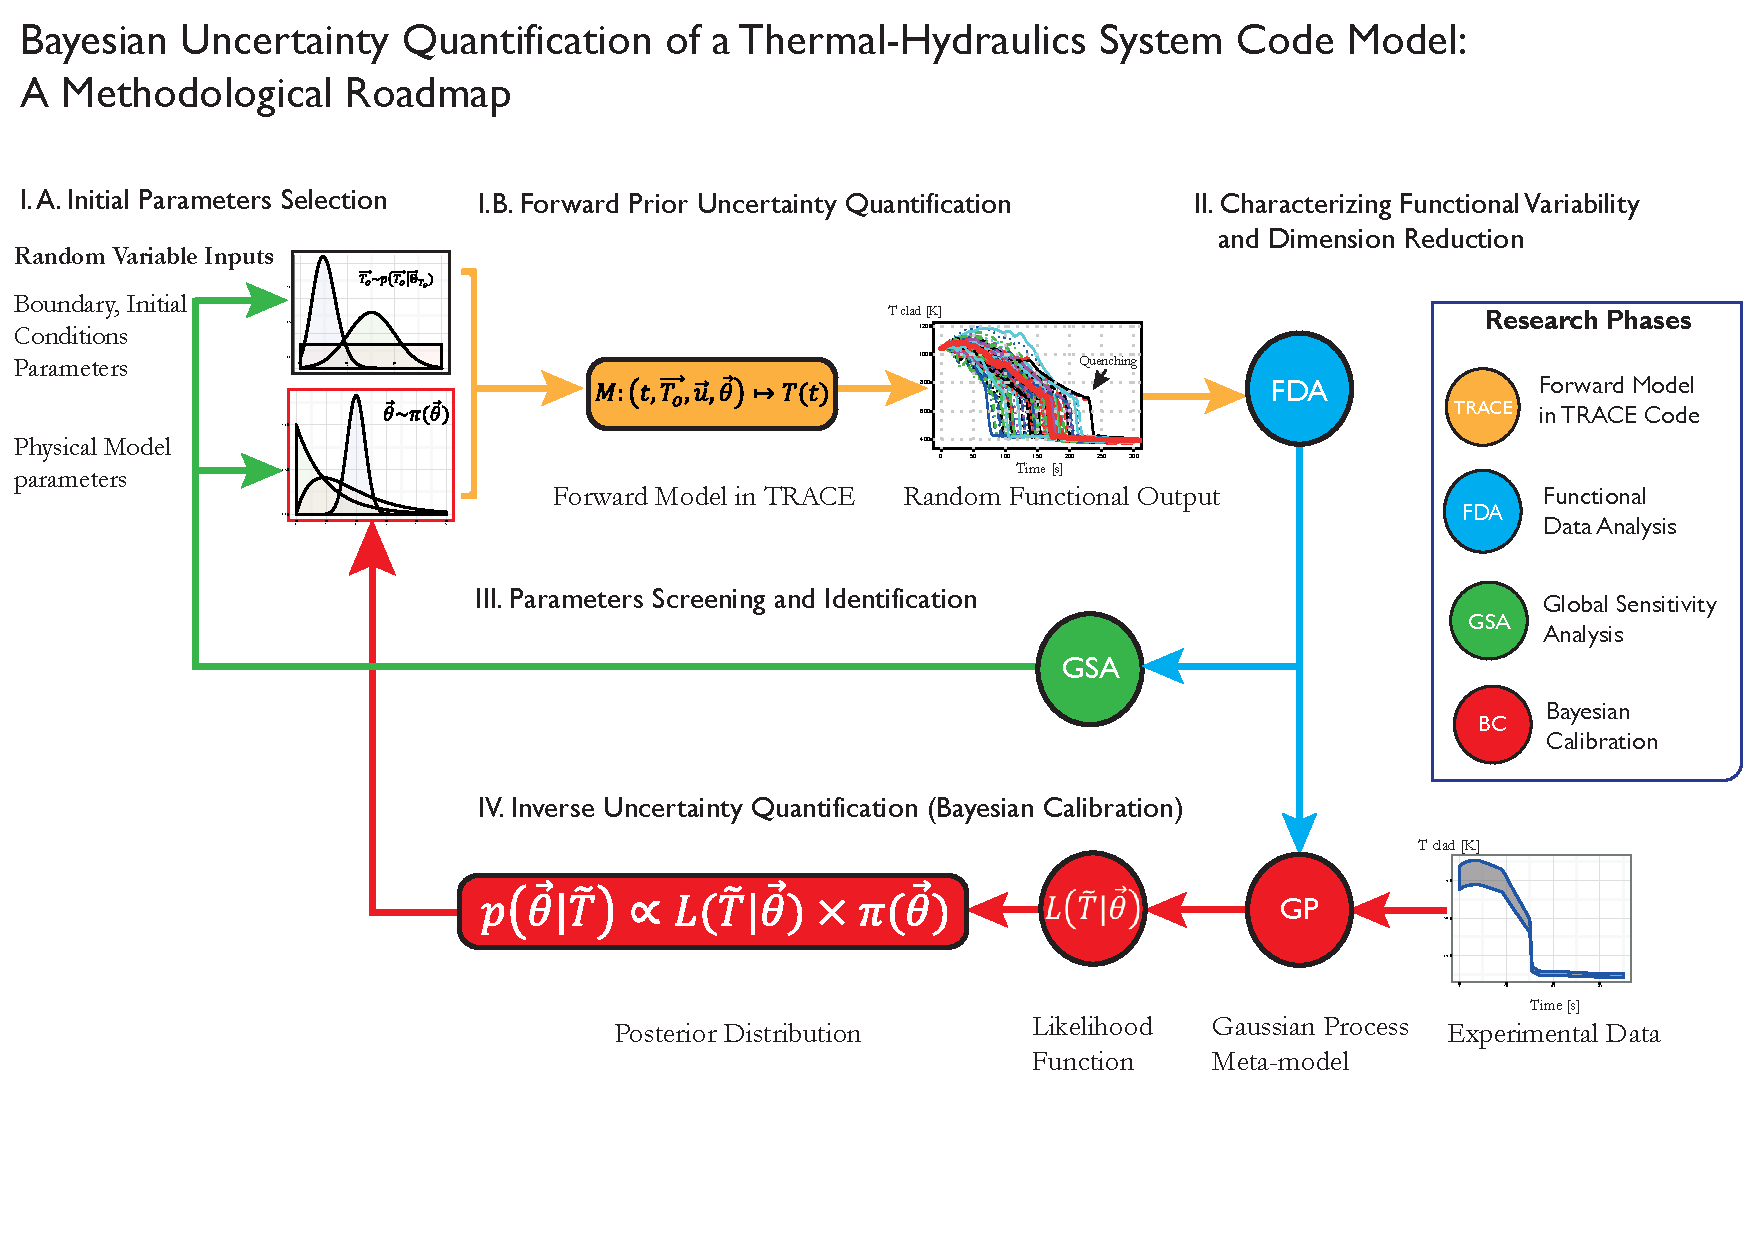
\includegraphics[width=0.85\textwidth]{../figures/methodologicalRoadmap/methodologicalRoadmap.pdf}
%	\caption{Methodological Roadmap of the Thesis}
%	\label{fig:methodological_roadmap}
%\end{sidewaysfigure}